\subsubsection{Descripci\'on} 
\textbf{A tableaux-like method to infer all minimal keys
P.CORDERO,M.ENCISO,A.MORA and I.PEREZ DE GUZMAN,
Logic Journal of the IGPL, Volume 22, Issue 6, 1 December 2014, Pages 1019 1044}

\cite{Reduction}
Este algoritmo busca resolver el problema de la b\'usqueda de claves lo mas eficientemente posible. Para ello trata de simplificar lo m\'aximo posible el conjunto de implicaciones del cual se quieren obtener las claves, aplicando la l\'ogica de simplificaciones.

Se van a definir algunos conceptos que servir\'an de ayuda a la hora de entender el algoritmo desarrollado.\\

\textbf{Core y Body}

Siendo \(\Omega\) un conjunto de atributos, \(\Gamma\) un conjunto de implicaciones sobre \(\Omega\), definimos el core y el body de \(\Gamma\) como:
\begin{center}
    \(core(\Omega,\Gamma) = \Omega \setminus \big(\bigcup_{\substack{A \to B \in \Gamma}} B\big)\)

    \(body(\Omega,\Gamma) = \big(\bigcup_{\substack{A \to B \in \Gamma}} A\big) \setminus (core(\Omega,\Gamma))^+\)
\end{center}
Ambos permitir\'an simplificar \(\Gamma\) y as\'i agilizar el proceso de obtenci\'on de las claves. Adem\'as se tiene que, si \(K\) es una clave minimal, cumple que 
\begin{center}
    \(core(\Omega,\Gamma) \subseteq K \subseteq core(\Omega,\Gamma) \cup body(\Omega,\Gamma)\)
\end{center}
\newpage
\subsubsection{C\'odigo} 
\lstinputlisting{r_code/reduction.method.R}
\newpage
\subsubsection{Ejemplo} 
\begin{figure}[H]
    \centering
    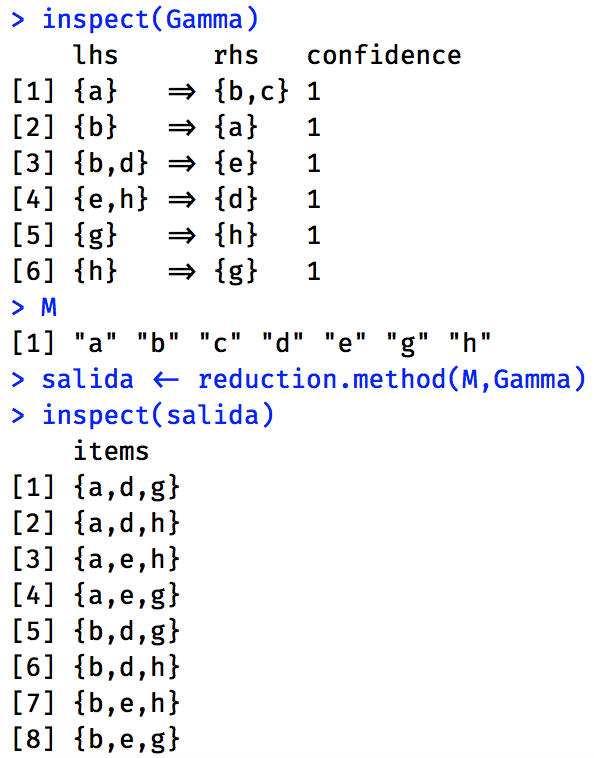
\includegraphics[scale=0.75]{reduction_1}
    \caption{Ejemplo Reduction}
    \label{fig:reduction_1}
\end{figure}
\subsubsection{Comparativa/Versiones} 